\section{MARCO PRÁCTICO E IMPLEMENTACIÓN TÉCNICA}

El marco práctico constituye el núcleo de ingeniería del proyecto, integrando los módulos de recolección resiliente de datos, el pipeline multimedia, la arquitectura de base de datos serverless y las interfaces ciudadanas desplegadas.

\subsection{Ingeniería de Extracción Resiliente (Web Content Mining)}

\subsubsection{Scraper Hipermaxi: Evasión de Radware y Detección de Scroll Infinito}
El portal de Hipermaxi (\url{https://www.hipermaxi.com}) está construido como una aplicación de una sola página en Angular protegida por el WAF corporativo \textbf{Radware Bot Manager}. Para operar sobre este entorno sin interrupciones, el script \texttt{scraper\_hipermaxi.mjs} implementa una estrategia de conexión basada en \textbf{contextos persistentes de usuario} (\textit{Persistent Context}) mediante Playwright:

\begin{enumerate}[leftmargin=*]
    \item \textbf{Persistencia de Sesión y Cookies:} El navegador Chromium se inicializa vinculando el directorio local \texttt{.browser\_profile\_hipermaxi}. Esto permite que las cookies de sesión y los tokens de verificación resueltos por un operador humano persistan a través de múltiples ejecuciones, eludiendo la necesidad de resolver desafíos en cada ciclo de ingesta.
    \item \textbf{Detección y Sondeo Activo de WAF:} El crawler monitorea de forma continua la presencia de títulos y contenedores del WAF (\textit{``Radware Bot Manager''}, \textit{``Human Verification''}). En caso de dispararse un desafío hCAPTCHA, el script ejecuta una rutina de sondeo activo (\texttt{pollForHumanBypass}) que pausa temporalmente la extracción, notifica al operador y reanuda el scraping de manera automática tan pronto como se restablece la navegación regular.
    \item \textbf{Sincronización con Scroll Infinito:} El catálogo de productos no utiliza paginación tradicional sino desplazamiento vertical asíncrono. Al desplazarse hacia la parte inferior de la vista, la aplicación inyecta en el DOM el selector dinámico \texttt{span:has-text("Obteniendo más productos")} acompañado de una animación giratoria (\textit{spinner}). El scraper ejecuta ciclos de scroll controlado (\texttt{window.scrollBy(0, 1200)}) sincronizados con la desaparición del indicador de carga y el incremento en el recuento de tarjetas de producto (\texttt{div.product-item}), deteniéndose únicamente cuando transcurren más de tres ciclos consecutivos sin nuevas inserciones en el DOM (véanse los selectores detallados en la Tabla~\ref{tab:anexo_selectores} del Anexo C).
\end{enumerate}

El agente recorre de manera parametrizada las \textbf{29 sucursales} activas del eje central boliviano (12 en La Paz, 11 en Santa Cruz y 6 en Cochabamba) y cubre las \textbf{32 categorías} estructuradas (19 de supermercado y 13 de farmacia).

\subsubsection{Scraper Farmacorp: Paginación Numérica en Shopify}
La plataforma de Farmacorp (\url{https://farmacorp.com}) opera sobre el motor de comercio electrónico Shopify bajo el tema corporativo Empire. A diferencia de esquemas con scroll infinito, Shopify segmenta sus colecciones mediante controles de paginación numérica tradicional (\texttt{nav.pagination}).

Para maximizar la densidad y estabilidad de la extracción, el crawler fuerza la vista en cuadrícula añadiendo el parámetro de consulta \texttt{?page=N\&grid\_list=grid-view}. El script inspecciona el último elemento enlace dentro de \texttt{nav.pagination} para determinar el número total de páginas de cada colección. Si una colección contiene 45 páginas, el crawler genera la secuencia de peticiones de manera controlada, extrayendo de cada tarjeta el título del producto, la marca o laboratorio, el precio regular, el precio con descuento promocional y el enlace canónico. El agente procesa de forma recursiva más de \textbf{70 colecciones oficiales} organizadas en las macro-áreas de Salud y Medicamentos, Belleza, Cuidado Personal, Mamá y Bebé, y Cuidado del Hogar (Tabla~\ref{tab:enlaces_retail}).

\subsubsection{Scraper Farmacias Chávez: Decodificación de Paginación Ant Design}
Farmacias Chávez (\url{https://www.farmaciaschavez.com.bo}) implementa una arquitectura moderna con renderizado del lado del servidor en Next.js y componentes visuales provistos por la librería Ant Design. El componente de navegación paginada no despliega una lista completa de números de página, sino un paginador compacto denominado \textbf{Simple Pagination} (\texttt{.ant-pagination-simple-pager}).

El script \texttt{scraper\_chavez.mjs} extrae el total de páginas evaluando una expresión regular sobre el contenido textual del elemento: \texttt{/\textbackslash/\textbackslash s*(\textbackslash d+)/}. Al obtener el número total (por ejemplo, 44 páginas en la categoría de medicamentos), el agente recorre secuencialmente las URLs parametrizadas o activa programáticamente el botón de avance (\textit{next chevron}) esperando la hidratación del nuevo lote de productos.

Adicionalmente, el scraper recorre el menú de departamentos y familias de productos, clasificando los medicamentos frente a un diccionario especializado de más de 40 fármacos esenciales de la farmacopea boliviana (Paracetamol, Amoxicilina, Omeprazol, Losartán, etc.) y más de 35 laboratorios farmacéuticos nacionales e internacionales (Laboratorios INTI, Droguería INTI, Bagó, Cofar, Terbol, Crespal, Vita, Bayer, Roemmers, etc.).

\subsection{Pipeline Multimedia y Persistencia en Neon Object Storage S3}
Las imágenes de productos hospedadas en plataformas de comercio electrónico suelen servirse a través de rutas de proxy efímeras (como \texttt{/\_next/image?url=...}) o enlaces con parámetros de firma que caducan periódicamente. Para evitar la pérdida de activos visuales y eliminar la dependencia de servidores externos, se implementó el pipeline de sincronización multimedia \texttt{sync\_images\_to\_s3.mjs}:

\begin{enumerate}[leftmargin=*]
    \item \textbf{Desempaquetado de Proxies:} El script inspecciona las URLs de imagen recolectadas, extrayendo el enlace fuente absoluto subyacente.
    \item \textbf{Descarga y Normalización Concurrente:} Utilizando un pool de concurrencia de 5 trabajadores asíncronos con cabeceras de emulación de navegador, las imágenes se descargan en memoria y se convierten a formato WebP o PNG normalizado.
    \item \textbf{Carga a Neon Object Storage S3:} Los archivos se suben al bucket \texttt{assets} estructurados bajo el prefijo \texttt{assets/products/\{cadena\}/\{sku\_hash\}.webp}.
    \item \textbf{Proxy de Streaming y Caché:} La plataforma web Next.js expone el endpoint \texttt{/api/storage/[...key]}, el cual transmite las imágenes vía streaming hacia el cliente incorporando la cabecera HTTP \texttt{Cache-Control: public, max-age=604800, immutable}, garantizando tiempos de carga inferiores a 25 milisegundos en peticiones recurrentes.
\end{enumerate}

\subsection{Arquitectura de Base de Datos y Triggers Reactivos en Neon Serverless}

\subsubsection{Modelo Estrella y Particionamiento Temporal}
La persistencia de los datos se configuró en \textbf{Neon Serverless PostgreSQL} implementando un modelo estrella que disocia los datos dimensionales estáticos de los eventos transaccionales dinámicos:

\begin{itemize}[leftmargin=*]
    \item \textbf{Catálogo Maestro (\texttt{catalogo\_productos\_master}):} Almacena la definición inmutable de cada producto identificado por su clave primaria \texttt{sku\_id}. Contiene atributos como nombre canónico, cadena comercial, departamento, sucursal, categoría, laboratorio fabricante, forma farmacéutica y enlace canónico persistente.
    \item \textbf{Histórico de Precios Particionado (\texttt{precios\_historico}):} Diseñada como una tabla de series temporales particionada de forma declarativa por rangos de fecha (\texttt{PARTITION BY RANGE (fecha)}). Cada partición aloja un mes calendario de observaciones (por ejemplo, \texttt{precios\_historico\_2026\_11}). Las consultas sobre rangos de fecha específicos ejecutan \textit{partition pruning}, descartando las tablas secundarias que no corresponden a la ventana temporal consultada y reduciendo drásticamente el consumo de memoria I/O.
    \item \textbf{Consolidación Semanal Fría (\texttt{precios\_historico\_semanal}):} Almacena agregaciones analíticas (precio mínimo, máximo, promedio ponderado y precio de cierre) por SKU, año y semana, reduciendo en un 85.7\% el espacio de almacenamiento para análisis macroeconómicos longitudinales.
\end{itemize}

\subsubsection{Resolución de Triggers Reactivos y Desacoplamiento de Esquemas}
Durante el desarrollo del sistema, las inserciones masivas de productos de supermercado hacia la tabla operativa \texttt{canasta\_precios} experimentaron fallos HTTP 400 en Neon debido a una colisión en la función unificada original de disparadores:
\begin{quote}
    \footnotesize\texttt{ERROR 42703: record "new" has no field "precio\_anterior\_bs" en PL/pgSQL function fn\_replicate\_to\_master\_and\_history()}
\end{quote}

Este error se originaba porque la tabla operacional \texttt{canasta\_precios} maneja una estructura simplificada (sin campos de descuento previo), mientras que \texttt{medicamentos\_precios} sí incluye \texttt{precio\_anterior\_bs} y \texttt{descuento\_pct}. La invocación de un trigger compartido provocaba que la referencia a \texttt{NEW.precio\_anterior\_bs} causara un fallo de compilación en tiempo de ejecución para las filas provenientes de la canasta básica.

La solución arquitectónica definitiva consistió en **desacoplar completamente la lógica reactiva** en dos procedimientos independientes mediante el script \texttt{fix\_triggers.mjs}:
\begin{enumerate}[leftmargin=*]
    \item \texttt{fn\_replicate\_canasta\_to\_master()}: Asociada exclusivamente a \texttt{canasta\_precios}. Gestiona el \texttt{UPSERT} sobre \texttt{catalogo\_productos\_master} mapeando \texttt{fuente} como categoría/sucursal y calcula los deltas de precio en \texttt{precios\_historico} sin acceder a atributos inexistentes.
    \item \texttt{fn\_replicate\_medicamento\_to\_master()}: Asociada exclusivamente a \texttt{medicamentos\_precios}. Mapea \texttt{cadena}, \texttt{laboratorio} y \texttt{presentacion}, computando de forma nativa los descuentos relativos y preservando el estado de disponibilidad del fármaco.
\end{enumerate}

\subsubsection{Justificación Técnica del Diagrama Entidad-Relación Físico}
En la Figura~\ref{fig:neon_er_diagram} se exhibe el diagrama físico de las 10 tablas activas del sistema, capturado directamente desde la consola administrativa de Neon Serverless PostgreSQL.

\begin{figure}[htbp]
    \centering
    \caption{Diagrama Entidad-Relación Físico de las 10 Tablas en Neon Serverless PostgreSQL}
    \label{fig:neon_er_diagram}
    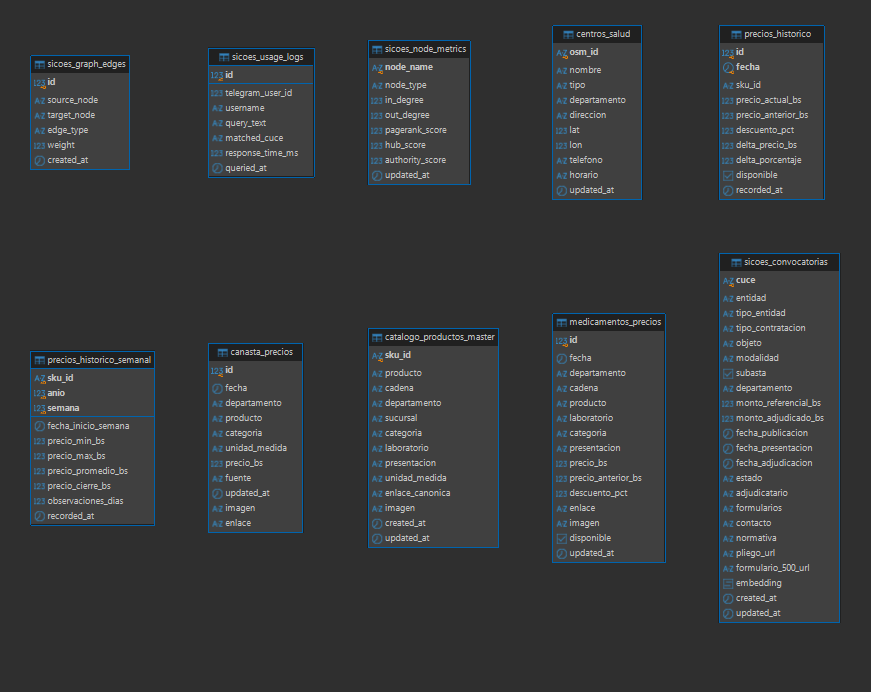
\includegraphics[width=0.92\linewidth]{figuras/neon_db_er_diagram_real.png}
    \figurenote{Esquema físico relacional en la consola de Neon. Comprende las tablas de precios (\texttt{canasta\_precios}, \texttt{medicamentos\_precios}), el catálogo maestro (\texttt{catalogo\_productos\_master}), el histórico particionado (\texttt{precios\_historico}, \texttt{precios\_historico\_semanal}), los centros de salud (\texttt{centros\_salud}), el grafo SICOES (\texttt{sicoes\_graph\_edges}, \texttt{sicoes\_node\_metrics}), las convocatorias vectorizadas (\texttt{sicoes\_convocatorias}) y los registros de uso del bot (\texttt{sicoes\_usage\_logs}).}
\end{figure}

Un aspecto de especial interés en la Figura~\ref{fig:neon_er_diagram} es que las tablas se visualizan como entidades independientes, sin líneas físicas explícitas de claves foráneas (\textit{Foreign Keys} - FK). Esta decisión de diseño responde a fundamentos rigurosos de ingeniería de bases de datos de alto rendimiento y modelos serverless:

\begin{enumerate}[leftmargin=*]
    \item \textbf{Restricciones de Particionamiento en PostgreSQL:} La tabla central de series de tiempo (\texttt{precios\_historico}) está particionada declarativamente por rango de fechas. En PostgreSQL, las restricciones de clave foránea directas hacia tablas particionadas complejas o desde particiones hijas hacia tablas maestras imponen limitaciones de indexación y pueden inducir bloqueos globales de catálogo durante la creación dinámica de nuevas particiones mensuales.
    \item \textbf{Rendimiento de Inserción Masiva y Ausencia de Bloqueos (\textit{Locks}):} En pipelines de web scraping masivo, donde se insertan miles de filas de manera concurrente en lotes (\textit{bulk inserts}), las claves foráneas físicas forzarían una verificación síncrona fila por fila contra la tabla maestra, adquiriendo bloqueos compartidos (\textit{shared row locks}) que degradan severamente el rendimiento y pueden provocar interbloqueos (\textit{deadlocks}).
    \item \textbf{Garantía de Integridad Referencial Reactiva mediante Triggers:} La integridad referencial no se encuentra desatendida; está gobernada a nivel lógico y operacional por las funciones PL/pgSQL mencionadas. Cada vez que una fila ingresa a \texttt{canasta\_precios} o \texttt{medicamentos\_precios}, el trigger asegura automáticamente la existencia y sincronización del registro en \texttt{catalogo\_productos\_master} antes de insertar la observación en \texttt{precios\_historico}, garantizando consistencia absoluta sin penalizar la concurrencia.
\end{enumerate}

Para complementar la representación física de las tablas y transparentar la gobernanza relacional, la Figura~\ref{fig:er_logico_triggers} ilustra el modelo entidad-relación conceptual/lógico con la propagación reactiva de triggers hacia el catálogo maestro y la tabla de series temporales.

\begin{figure}[htbp]
    \centering
    \caption{Diagrama Entidad-Relación Lógico, Modelo Estrella y Triggers de Sincronización}
    \label{fig:er_logico_triggers}
    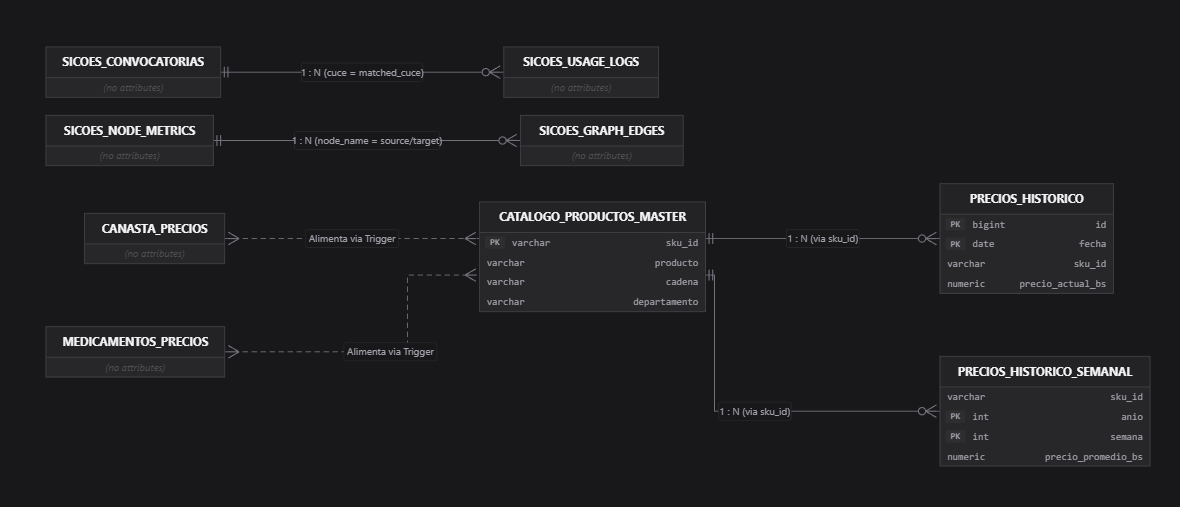
\includegraphics[width=0.95\linewidth]{figuras/imgER.png}
    \figurenote{Modelo relacional conceptual que ilustra la cardinalidad lógica (1:N) entre el catálogo maestro (\texttt{catalogo\_productos\_master}), el histórico particionado (\texttt{precios\_historico}) y las agregaciones semanales, gobernadas por los triggers reactivos desacoplados desde las tablas operacionales.}
\end{figure}

\clearpage
\subsection{Asistente Conversacional Telegram (Web Usage Mining)}
La interacción ciudadana ubicua se canaliza a través del bot oficial de Telegram \textbf{\texttt{@ChatDM7200bot}}, implementado mediante TypeScript y la librería Telegraf dentro del endpoint serverless \texttt{app/api/telegram/route.ts}.

\subsubsection{Arquitectura de Enrutamiento Telegraf y Teclados Interactivos Inline}
El asistente opera bajo un modelo reactivo basado en webhooks HTTPS seguros. Cuando el usuario interactúa con la interfaz móvil, el enrutador Telegraf clasifica la entrada distinguiendo mensajes textuales planos (\texttt{ctx.message.text}), comandos slash (\texttt{/start}, \texttt{/canasta}, \texttt{/medicamentos}, \texttt{/salud}, \texttt{/sicoes}) e interacciones con teclados en línea (\texttt{ctx.callbackQuery.data}). Como se aprecia en la Figura~\ref{fig:telegram_menu_sicoes}, la navegación inicial y la fiscalización del SICOES se estructuran mediante botones interactivos fluidos que no recargan el historial de chat.

\begin{figure}[htbp]
    \centering
    \caption{Vistas del Menú Principal y Módulo SICOES con IA en \texttt{@ChatDM7200bot}}
    \label{fig:telegram_menu_sicoes}
    \begin{minipage}{0.48\linewidth}
        \centering
        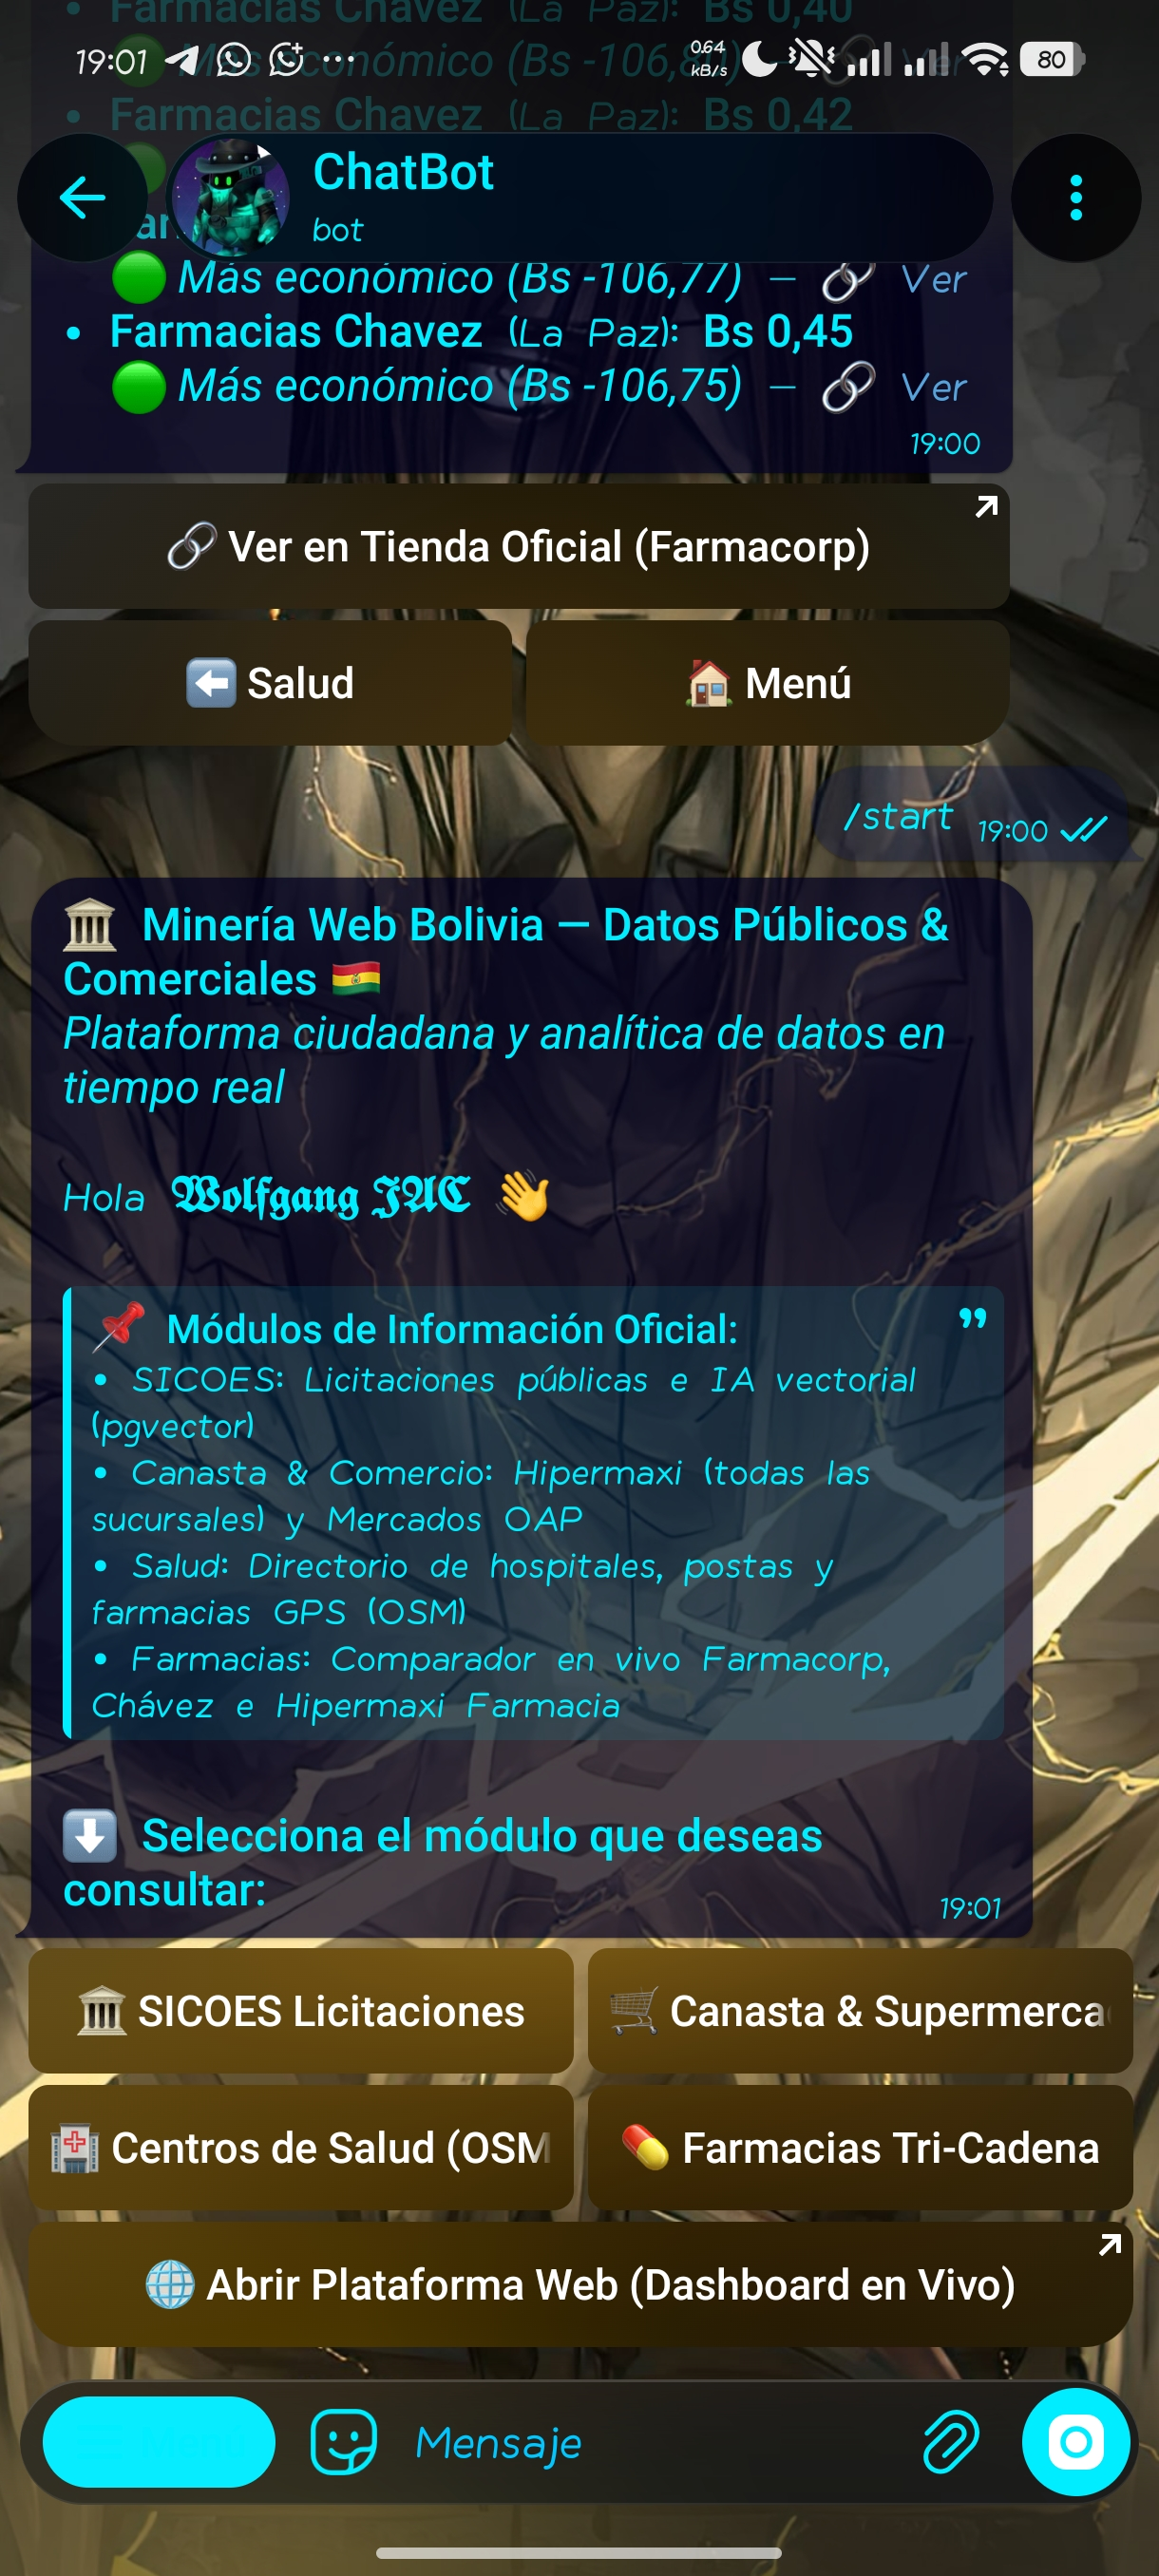
\includegraphics[height=10.5cm, keepaspectratio]{figuras/Screenshot_2026_11_15_19_01_07_813_org_telegram_messenger_web.jpg}
        \caption*{(a) Menú interactivo principal (\texttt{/start})}
    \end{minipage}\hfill
    \begin{minipage}{0.48\linewidth}
        \centering
        
\includegraphics[height=10.5cm, keepaspectratio]{figuras/Screenshot_2026_11_15_19_01_16_174_org_telegram_messenger_web.jpg}
        \caption*{(b) Módulo SICOES con IA (\texttt{/sicoes})}
    \end{minipage}
    \figurenote{Capturas de pantalla del bot de Telegram en producción móvil. (a) Menú principal con teclados en línea interactivos (\textit{Inline Keyboards}) hacia las áreas funcionales del sistema. (b) Módulo SICOES con búsqueda semántica asistida por IA y filtros facetados por estado y departamento.}
\end{figure}

\subsubsection{Módulos de Canasta Familiar y Comparador Tri-Cadena en Vivo}
Para el monitoreo de bienes de primera necesidad y la detección de asimetrías de precios en farmacias, el bot incorpora interfaces especializadas (Figura~\ref{fig:telegram_canasta_farmacia}):

\begin{figure}[htbp]
    \centering
    \caption{Vistas de Canasta Familiar y Comparador Tri-Cadena en \texttt{@ChatDM7200bot}}
    \label{fig:telegram_canasta_farmacia}
    \label{fig:telegram_pantallas_completas}
    \begin{minipage}{0.48\linewidth}
        \centering
        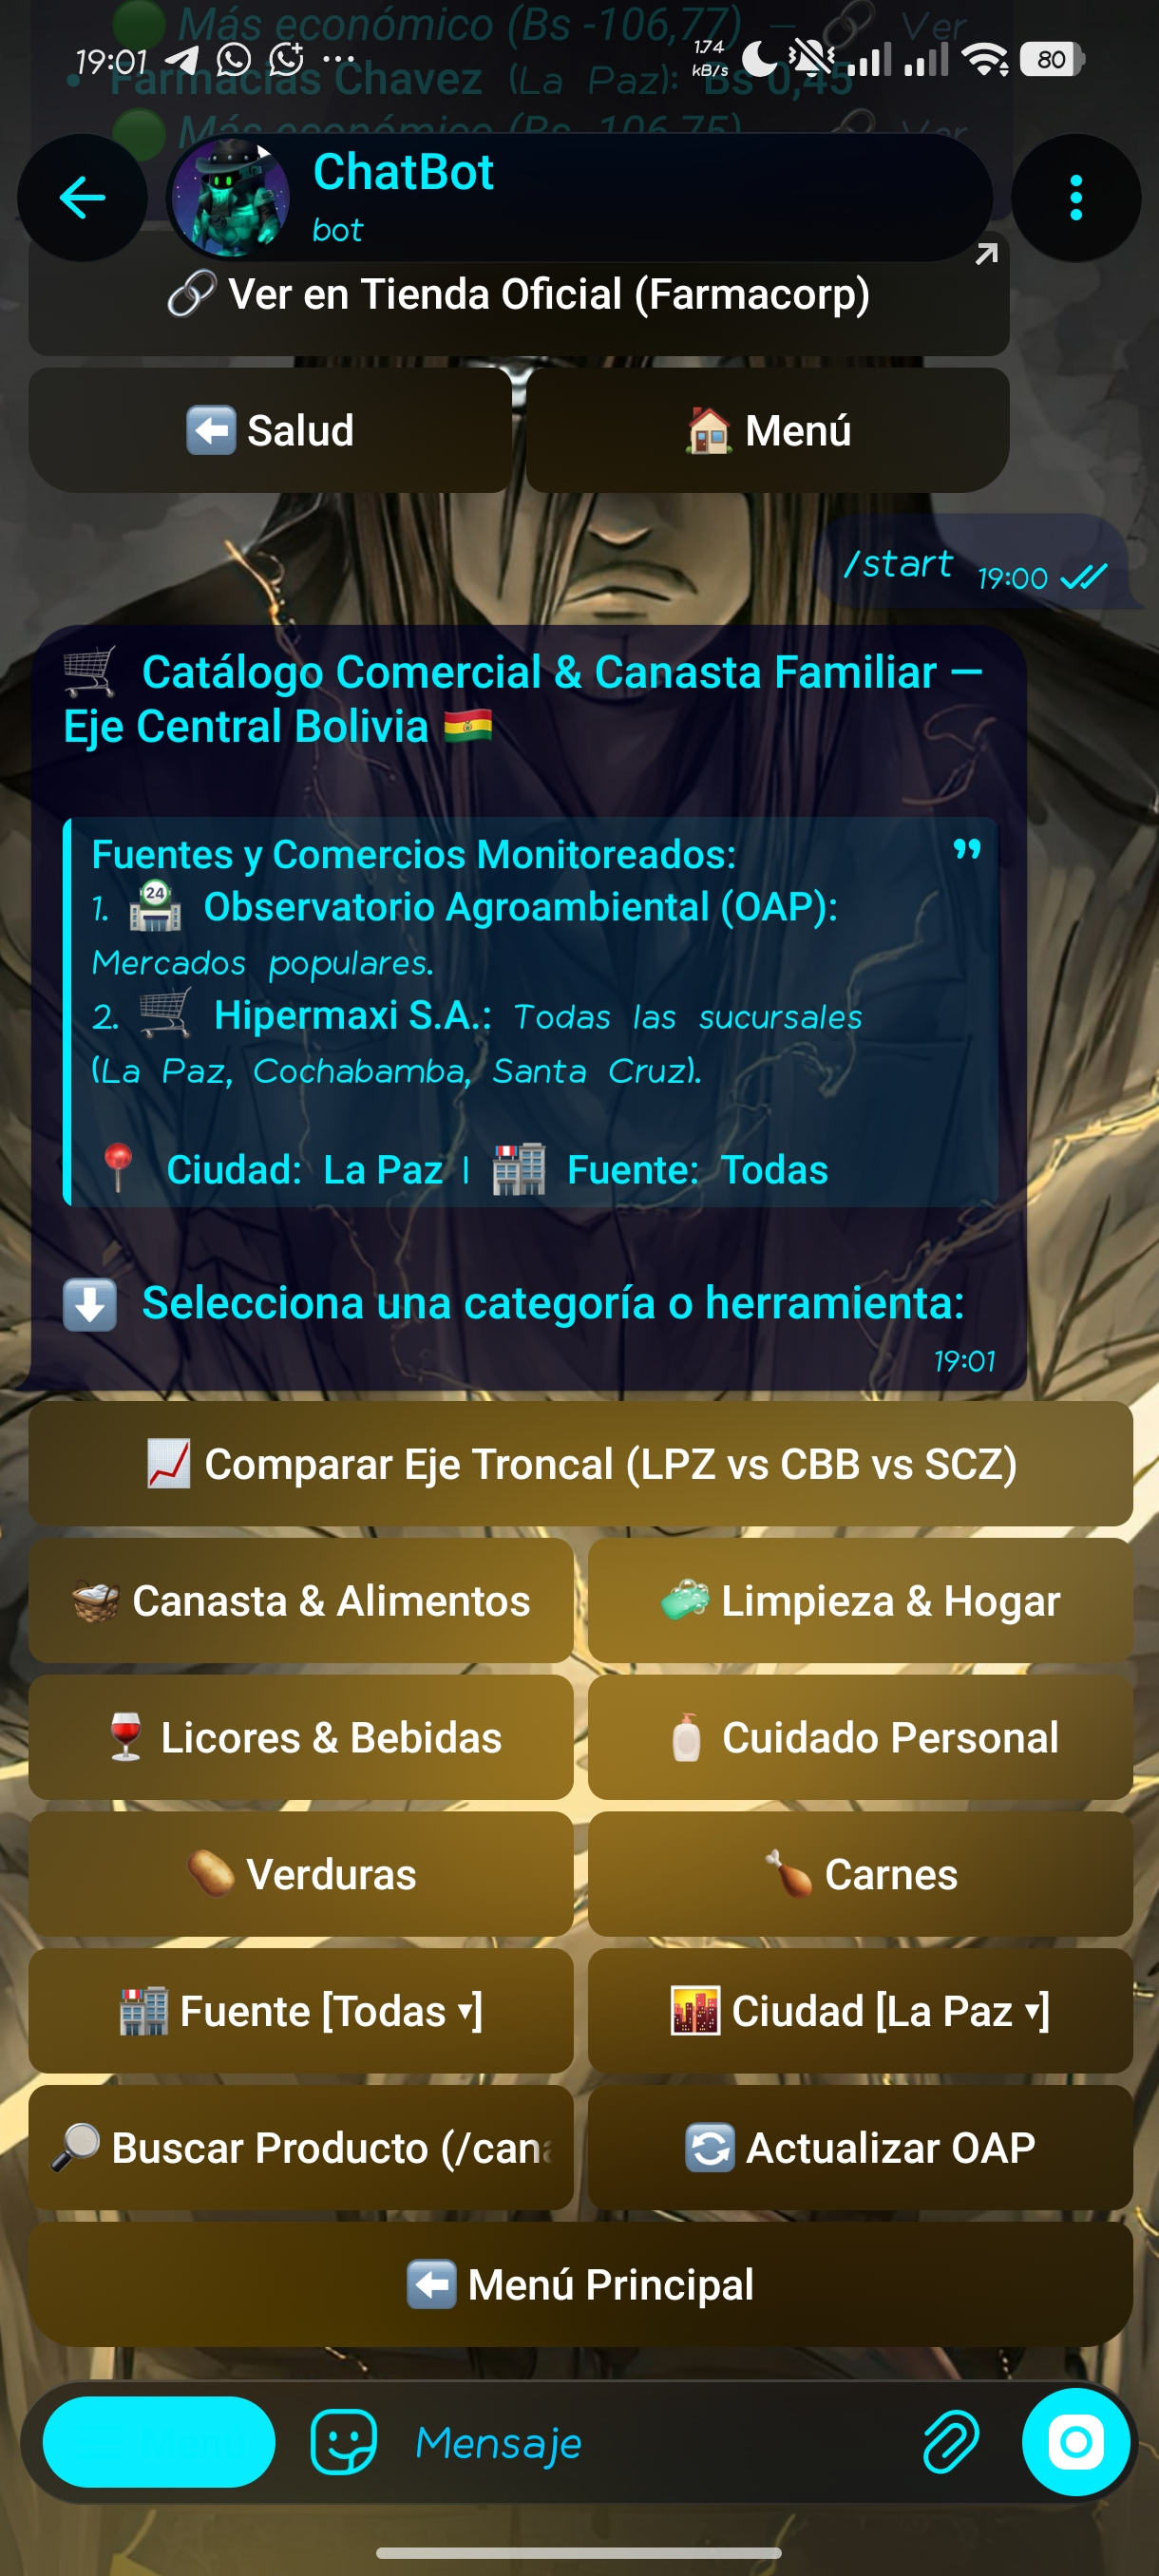
\includegraphics[height=10.5cm, keepaspectratio]{figuras/Screenshot_2026_11_15_19_01_23_015_org_telegram_messenger_web.jpg}
        \caption*{(a) Catálogo Canasta Familiar (\texttt{/canasta})}
    \end{minipage}\hfill
    \begin{minipage}{0.48\linewidth}
        \centering
        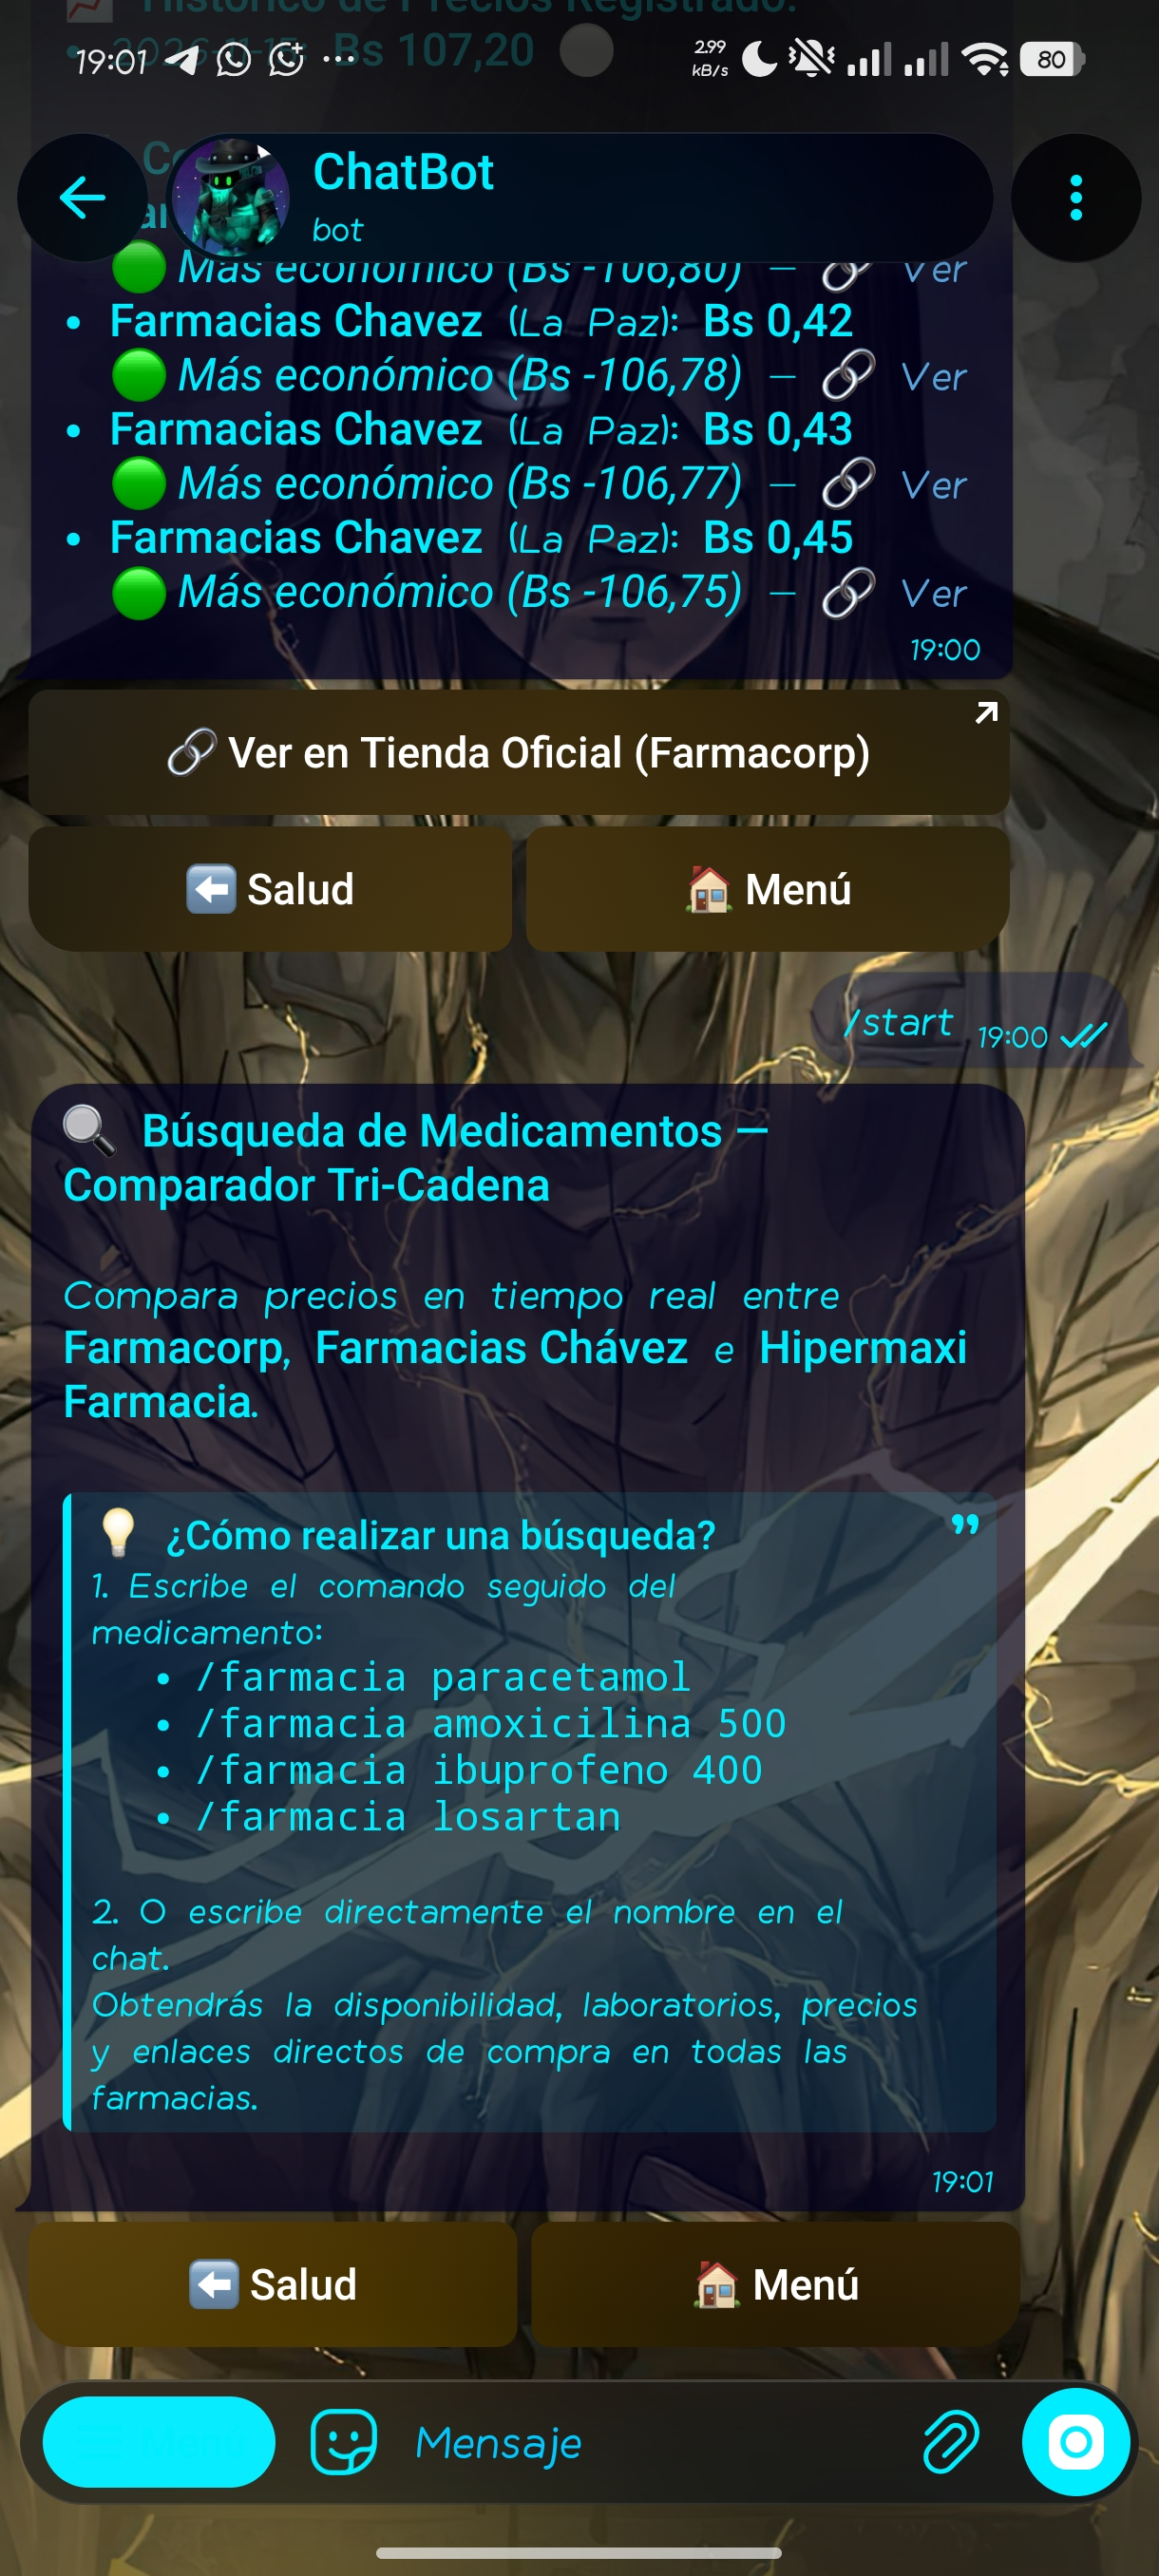
\includegraphics[height=10.5cm, keepaspectratio]{figuras/Screenshot_2026_11_15_19_01_32_006_org_telegram_messenger_web.jpg}
        \caption*{(b) Comparador tri-cadena en vivo (\texttt{/farmacia})}
    \end{minipage}
    \figurenote{Capturas de pantalla del asistente móvil en producción. (a) Exploración de macro-categorías comerciales de la canasta básica. (b) Comparativa simultánea de precios para Paracetamol 500 mg entre Farmacorp, Chávez e Hipermaxi Farmacia, detallando el ahorro monetario ($\Delta\text{Bs}$) y enlaces directos de auditoría ciudadana.}
\end{figure}

\clearpage
\subsubsection{Especificación de Comandos y Rutas Telegraf}
En la Tabla~\ref{tab:telegram_comandos} se sistematiza la especificación técnica de las rutas conversacionales del bot, documentando los manejadores del backend, las operaciones de persistencia subyacentes y las estructuras de respuesta ciudadana generadas.

\begin{table}[htbp]
    \centering
    \footnotesize
    \renewcommand{\arraystretch}{0.95}
    \setlength{\tabcolsep}{5pt}
    \caption{Especificación Técnica de Comandos, Rutas Telegraf y Respuestas Estructuradas en \texttt{@ChatDM7200bot}}
    \label{tab:telegram_comandos}
    \begin{tabularx}{\linewidth}{>{\raggedright\arraybackslash}p{2.5cm} >{\raggedright\arraybackslash}p{3.9cm} >{\raggedright\arraybackslash}p{4.7cm} L}
        \toprule
        \textbf{Comando / Evento} & \textbf{Manejador Telegraf} & \textbf{Operación en Base de Datos / Lógica} & \textbf{Estructura de Respuesta Generada} \\
        \midrule
        \texttt{/start} & \texttt{bot.start()} & Consulta de sesión y registro de usuario en \nolinkurl{sicoes_usage_logs}. & Menú interactivo principal con botones en línea (\textit{Inline Keyboard}) hacia Canasta, Medicamentos, Salud y SICOES. \\
        \addlinespace[3pt]
        \texttt{/canasta} \newline o texto libre & \texttt{bot.hears()} / \newline \texttt{on('text')} & \texttt{SELECT} con \texttt{ILIKE} sobre \nolinkurl{catalogo_productos_master} uniendo con \nolinkurl{canasta_precios}. & Tarjeta Markdown con desglose de precios en Hipermaxi, Farmacorp y Chávez, resaltando el precio mínimo y ahorro potencial ($\Delta\text{Bs}$). \\
        \addlinespace[3pt]
        \texttt{/medicamentos} & \texttt{bot.action(/med\_/)} & Búsqueda parametrizada sobre \nolinkurl{medicamentos_precios} filtrando por laboratorio y fármaco. & Comparativa farmacéutica multidimensional indicando presentación, descuento porcentual y enlaces canónicos directos de compra. \\
        \addlinespace[3pt]
        Envío de GPS \newline (\texttt{location}) & \texttt{bot.on('location')} & Ejecución de la fórmula geodésica de Haversine (Eq.~\ref{eq:haversine}) sobre tabla \nolinkurl{centros_salud}. & Lista ordenada de los 5 centros médicos más próximos al usuario, con distancia calculada en km, teléfono y dirección física. \\
        \addlinespace[3pt]
        \texttt{/sicoes} & \texttt{bot.command('sicoes')} & Búsqueda semántica vectorial (\texttt{pgvector}) con embeddings de 1024 dims sobre licitaciones. & Ficha ejecutiva de la convocatoria: CUCE, entidad licitante, objeto, monto referencial y puntaje de relevancia semántica. \\
        \addlinespace[3pt]
        Botón de Navegación & \texttt{bot.action('menu')} & Limpieza de estado transitorio de sesión y recarga de opciones principales. & Restablecimiento fluido del menú sin recrear el hilo del chat (\texttt{editMessageText}). \\
        \bottomrule
    \end{tabularx}
    \tablenote{Arquitectura de interacción ciudadana del asistente móvil. Cada evento registra de forma asíncrona la latencia y consulta en la tabla \texttt{sicoes\_usage\_logs} para Minería de Uso Web.}
\end{table}

\subsubsection{Manejo de Sesiones y Minería de Uso Web}
Cada interacción en el bot es interceptada por un middleware asíncrono que extrae el identificador anónimo del usuario (\texttt{user\_id}), el comando ejecutado, el término de búsqueda ingresado, el tiempo de procesamiento en milisegundos y la marca de tiempo UTC. Estos metadatos se persisten en la tabla \texttt{sicoes\_usage\_logs} en Neon PostgreSQL. Este mecanismo garantiza la trazabilidad operativa y proporciona el sustrato empírico para el análisis de Minería de Uso Web (\textit{Web Usage Mining}), permitiendo descubrir patrones de consulta, horarios de mayor concurrencia ciudadana y los medicamentos o productos de mayor interés social.

\subsection{Plataforma Web Interactiva en Next.js 14}
La plataforma web complementa al asistente móvil proveyendo una experiencia analítica enriquecida en pantallas de escritorio y dispositivos móviles:

\begin{enumerate}[leftmargin=*]
    \item \textbf{Panel de Filtros Facetados:} La vista \texttt{/canasta} incorpora controles de filtrado dinámico en cliente y servidor, permitiendo segmentar el catálogo por cadena comercial (Hipermaxi, Farmacorp, Chávez), departamento (La Paz, Santa Cruz, Cochabamba), rango de precios deslizante y disponibilidad de stock.
    \item \textbf{Catálogo Visual y Comparador:} Como se aprecia en la Figura~\ref{fig:web_catalogo}, cada tarjeta de producto expone su imagen optimizada servida vía streaming desde Neon S3, el precio unitario vigente, el precio anterior tachado, la insignia porcentual de ahorro y el botón de redirección hacia la tienda oficial de origen para auditoría ciudadana.
    \item \textbf{Módulo de Salud y Cartografía (\texttt{/salud}):} Integra un mapa dinámico con Leaflet que representa con marcadores de color diferenciado los hospitales de segundo y tercer nivel, centros integrales y farmacias de turno en la ciudad de La Paz.
\end{enumerate}

\begin{figure}[htbp]
    \centering
    \caption{Catálogo Visual de Productos de la Canasta Familiar con Precios y Enlaces Directos}
    \label{fig:web_catalogo}
    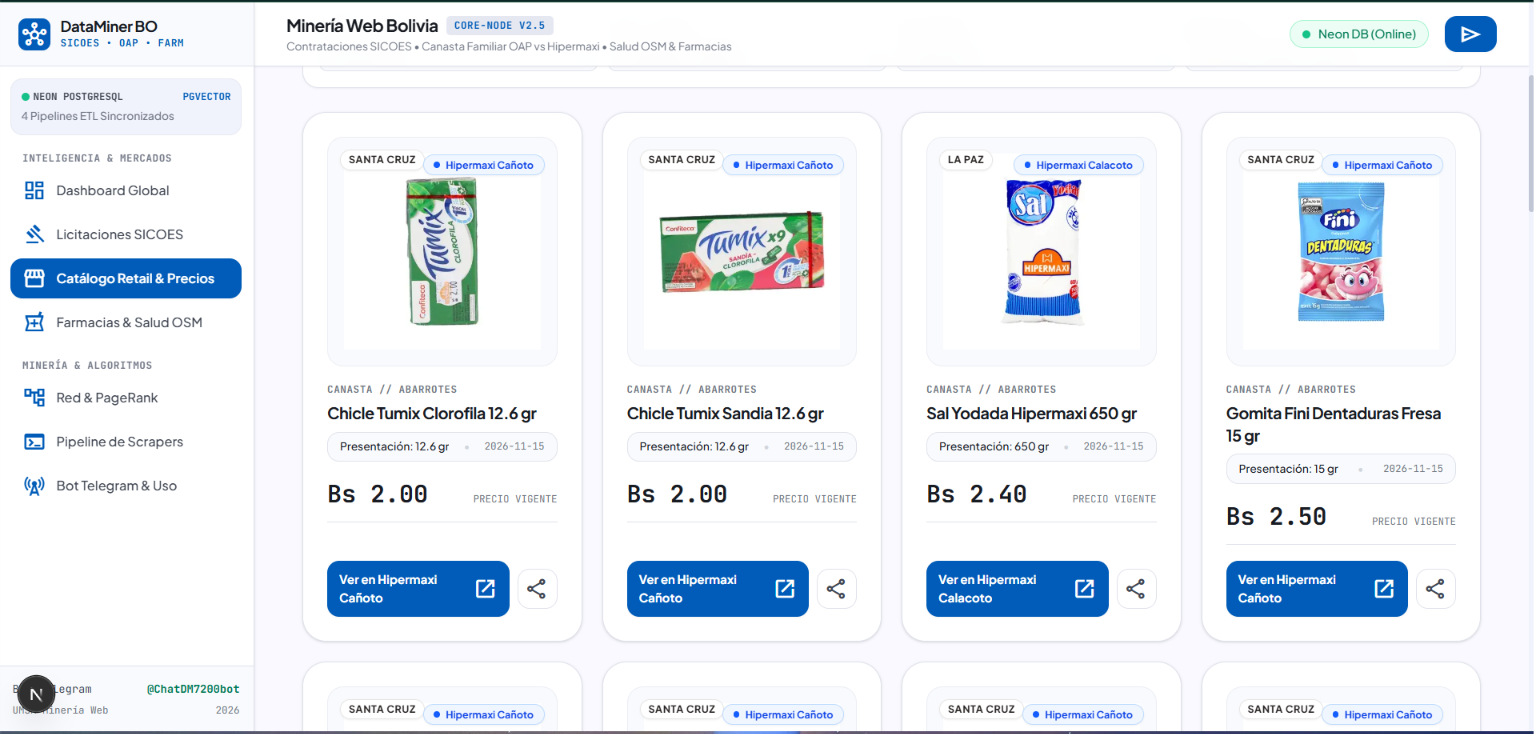
\includegraphics[width=0.92\linewidth]{figuras/imgListadoTienda.png}
    \figurenote{Vista del catálogo interactivo en Next.js 14 (\textit{DataMiner BO}). Exhibe las tarjetas de producto con imágenes optimizadas servidas vía streaming, segmentación multitienda (Hipermaxi Cañoto, Calacoto) y botones directos de auditoría ciudadana.}
\end{figure}
